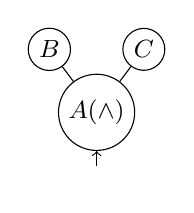
\begin{tikzpicture}[
    gate/.style={circle, draw, inner sep=2pt},
    every node/.style={font=\small}
]

% Inputs
\node (x1) at (0.6,0) {};

% XOR(x1,x2)
\node[gate] (xor12) at (0.6,0.8) {$A (\wedge)$};
\node[gate] (nodeb) at (0,1.6) {$B$};
\node[gate] (nodec) at (1.2,1.6) {$C$};
\draw (xor12) -- (nodeb);
\draw (xor12) -- (nodec);
\draw[->] (x1) -- (xor12);


\end{tikzpicture}
